%\documentclass[notes]{beamer}       % print frame + notes
%\documentclass[notes=only]{beamer}   % only notes
\documentclass{beamer}              % only frames
%
% Choose how your presentation looks.
%
% For more themes, color themes and font themes, see:
% http://deic.uab.es/~iblanes/beamer_gallery/index_by_theme.html
%
\mode<presentation>
{
  \usetheme{Madrid}      % or try Darmstadt, Madrid, Warsaw, ... default
  \usecolortheme{beaver} % or try albatross, beaver, crane, ... default
  \usefonttheme{default}  % or try serif, structurebold, ...
  \setbeamertemplate{navigation symbols}{}
  \setbeamertemplate{caption}[numbered]
} 

\usepackage[english]{babel}
\usepackage[utf8x]{inputenc}
\usepackage{caption}
\usepackage{booktabs}  % to make professional tables


\title[sip]{Group project}
%\subtitle{bla}
\author{Sandro Boccuzzo, No\" elle Schenk}
%\date{bla}


\begin{document}

{\usebackgroundtemplate{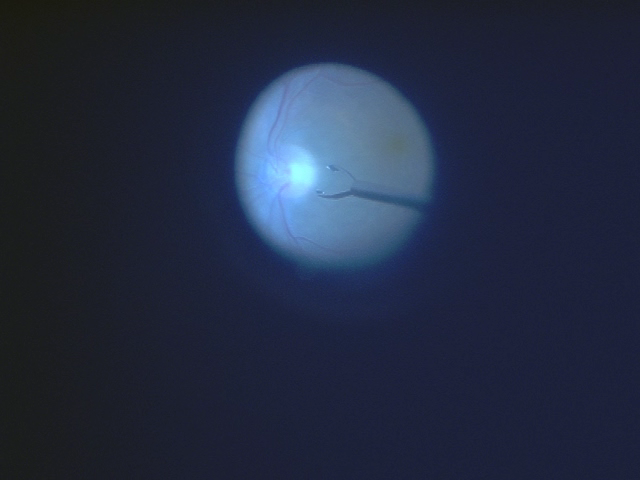
\includegraphics[width=1.0\paperwidth]{figs/title.png}}
  \begin{frame}
  \titlepage
  \end{frame} }



% ---------------------------------------------------------------------------------
\begin{frame}{simplest approach}
Filter with template cut around previous location. \\
\textbf{a}: time : 3.5 min / 100 images. Problem around picture a267:
\begin{figure}
    \centering
    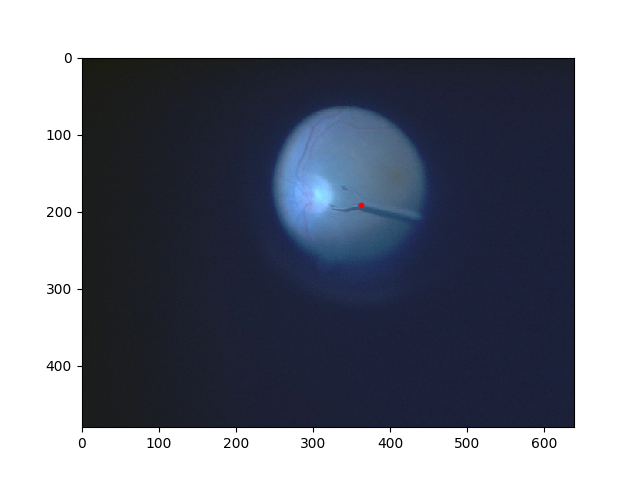
\includegraphics[width=0.25\textwidth]{figs/simplest/000267.png}
    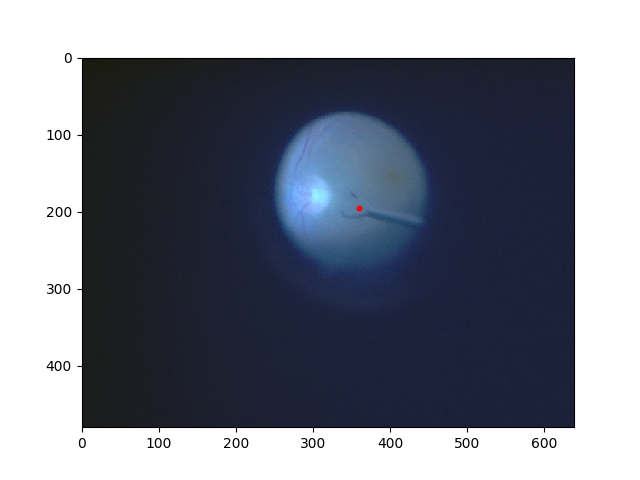
\includegraphics[width=0.25\textwidth]{figs/simplest/000268.png}
    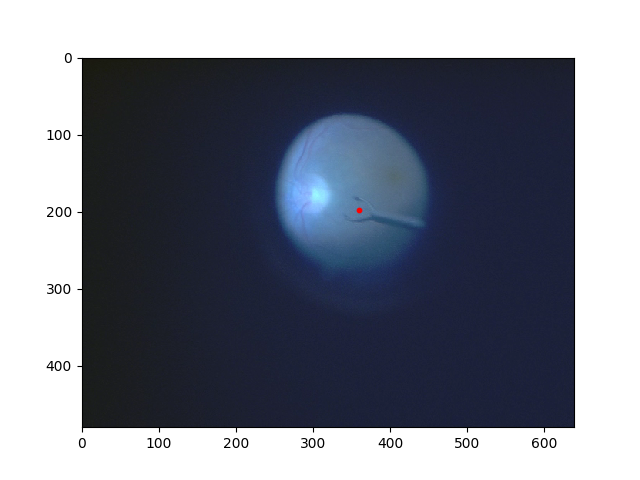
\includegraphics[width=0.25\textwidth]{figs/simplest/000269.png}
    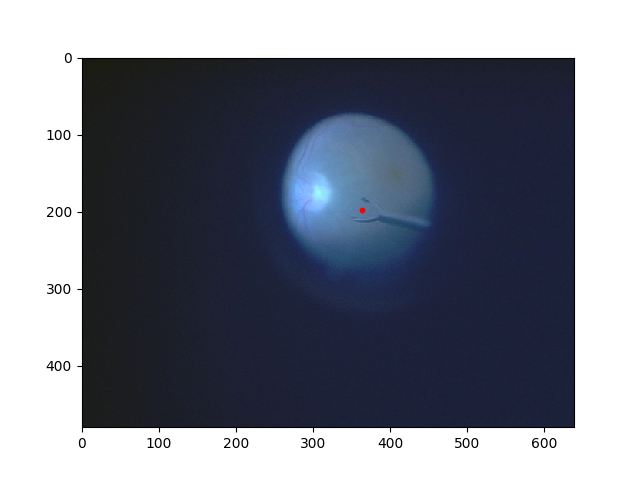
\includegraphics[width=0.25\textwidth]{figs/simplest/000270.png}
    
    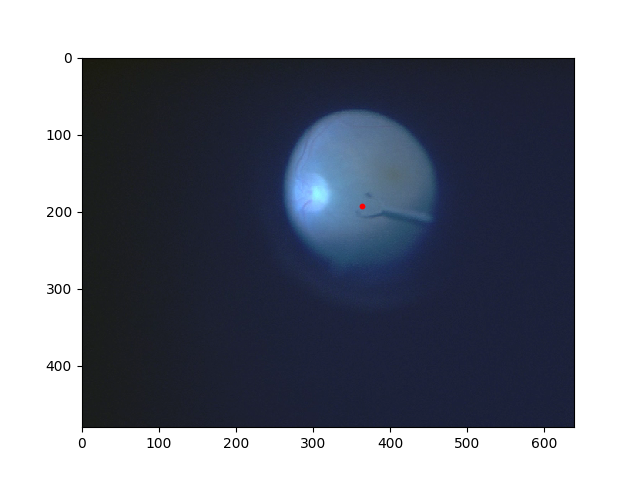
\includegraphics[width=0.25\textwidth]{figs/simplest/000271.png}
    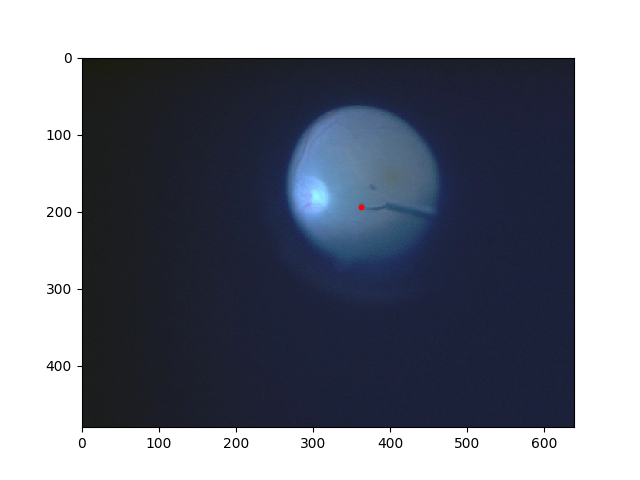
\includegraphics[width=0.25\textwidth]{figs/simplest/000272.png}
    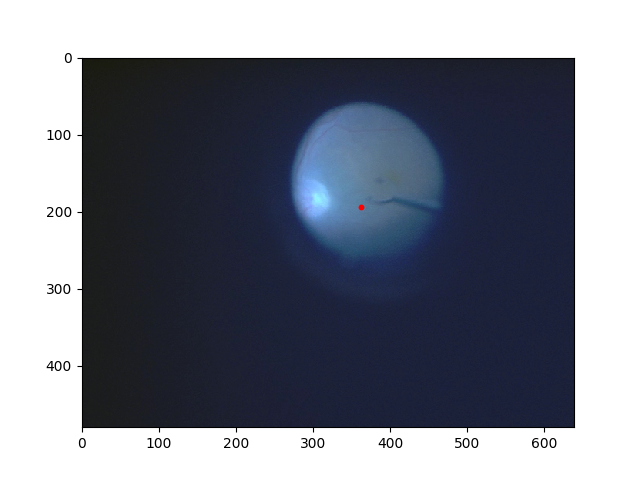
\includegraphics[width=0.25\textwidth]{figs/simplest/000273.png}
    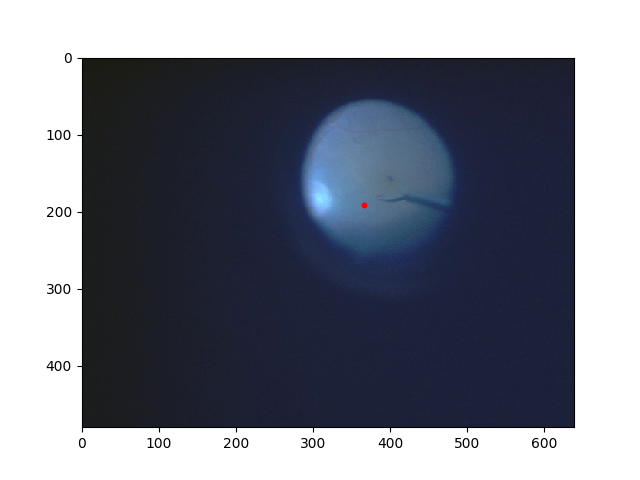
\includegraphics[width=0.25\textwidth]{figs/simplest/000274.png}
\end{figure}
\end{frame}

\begin{frame}{Only dominant color channel B}
Filter with template cut around previous location, only dominant color channel. \\
\textbf{b}: time : 23sec / 100 images. Problem around picture b1340:\\
point on tweezer, but not at branching point.
\begin{figure}
    \centering
    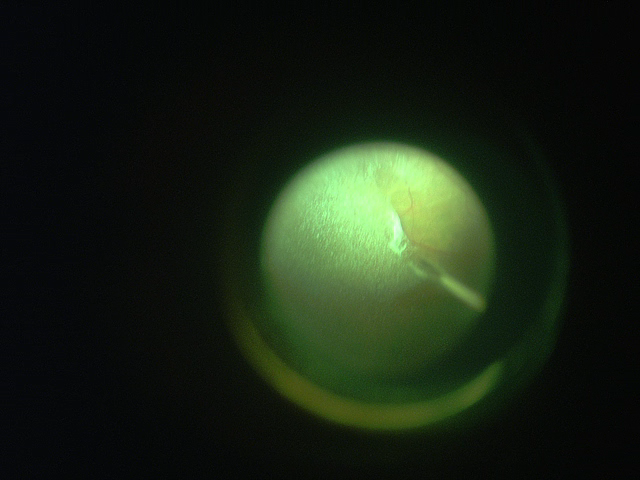
\includegraphics[width=0.25\textwidth]{figs/sw/001330.png}
    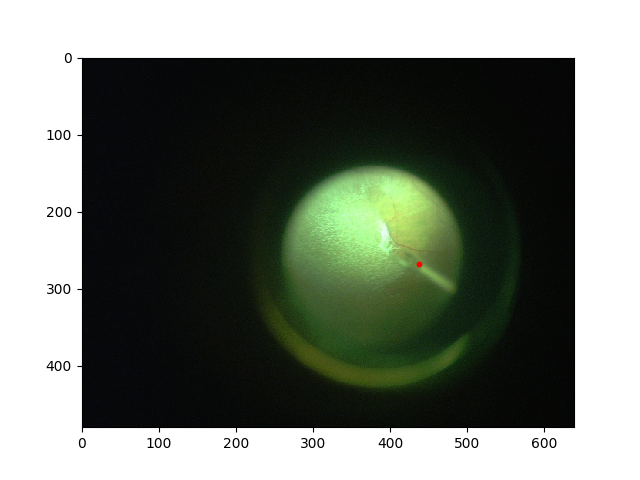
\includegraphics[width=0.25\textwidth]{figs/sw/001340.png}
    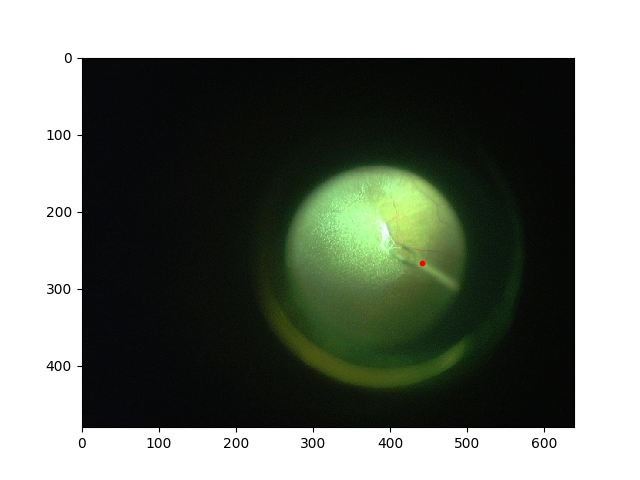
\includegraphics[width=0.25\textwidth]{figs/sw/001348.png}
    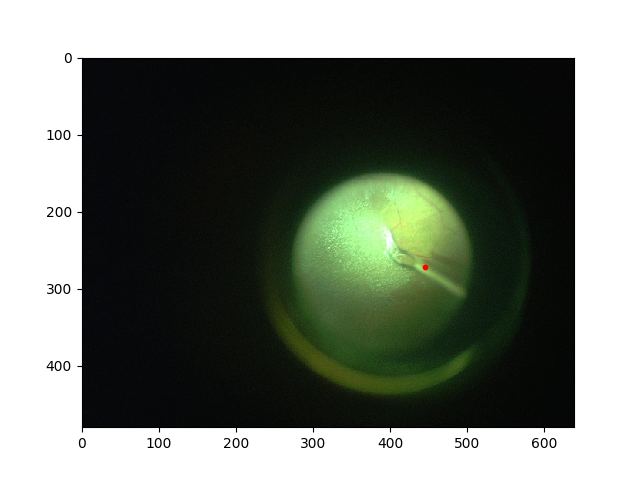
\includegraphics[width=0.25\textwidth]{figs/sw/001359.png}
    
    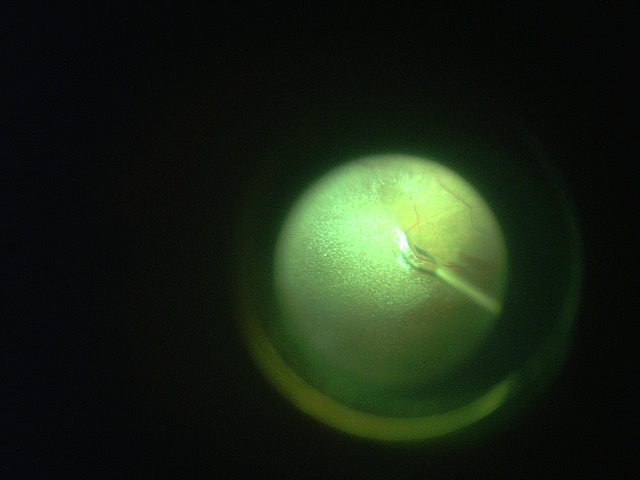
\includegraphics[width=0.25\textwidth]{figs/sw/001367.png}
    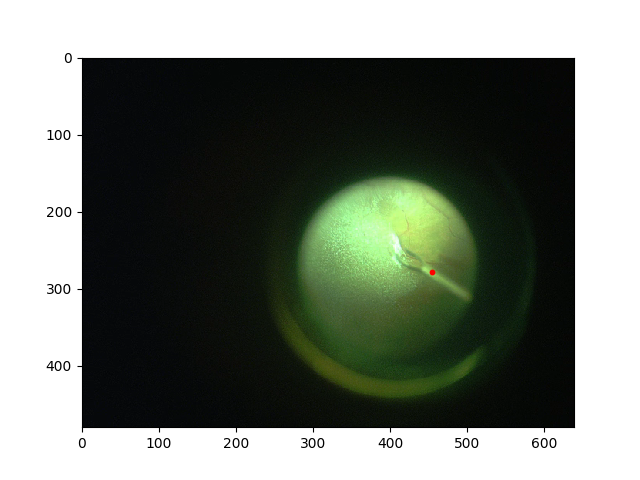
\includegraphics[width=0.25\textwidth]{figs/sw/001378.png}
    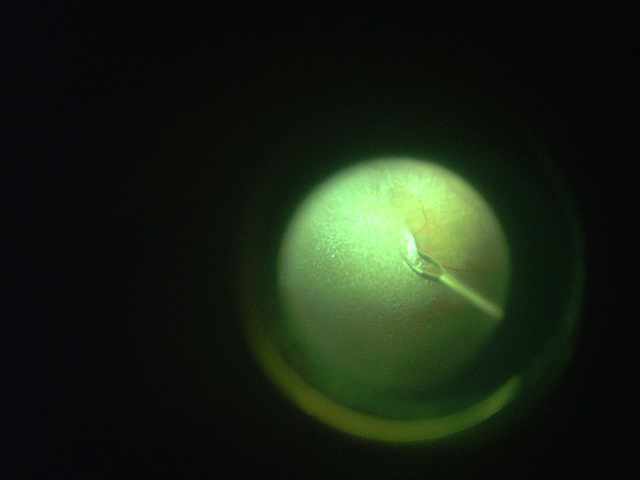
\includegraphics[width=0.25\textwidth]{figs/sw/001389.png}
    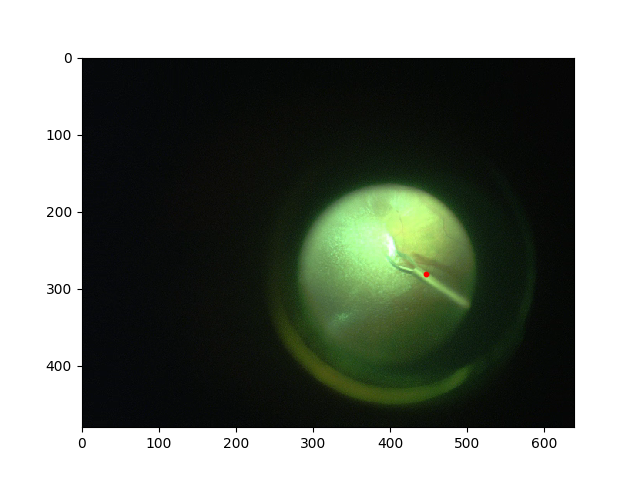
\includegraphics[width=0.25\textwidth]{figs/sw/001418.png}
\end{figure}
\end{frame}

\begin{frame}{Only dominant color channel A}
Filter with template cut around previous location, only dominant color channel. \\
\textbf{a}: time : 29sec / 100 images.\\
point lost tweezer, found point.
\begin{figure}
    \centering
    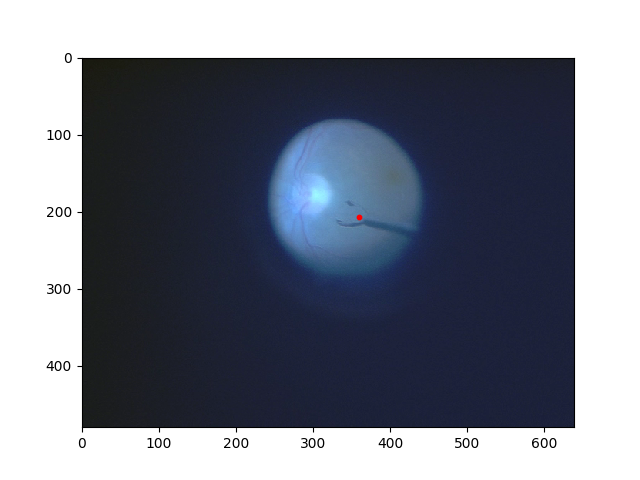
\includegraphics[width=0.25\textwidth]{figs/swa/000251.png}
    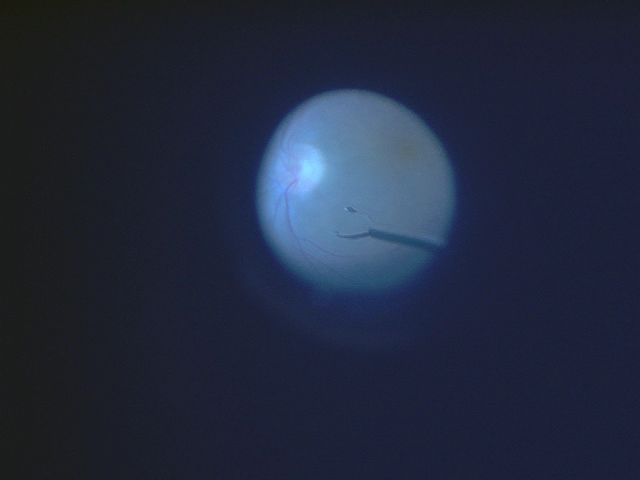
\includegraphics[width=0.25\textwidth]{figs/swa/000254.png}
    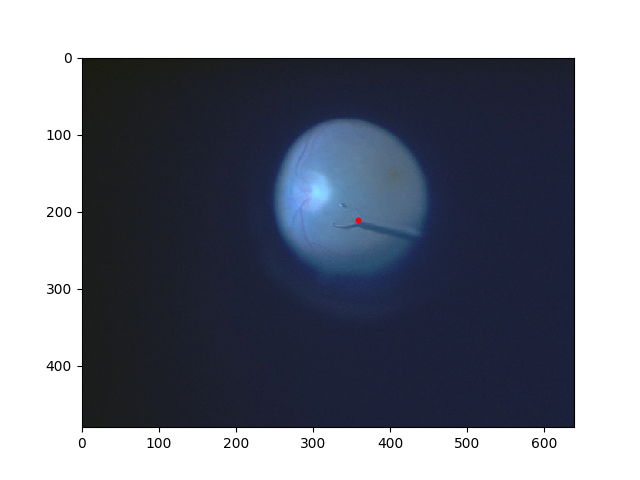
\includegraphics[width=0.25\textwidth]{figs/swa/000259.png}
    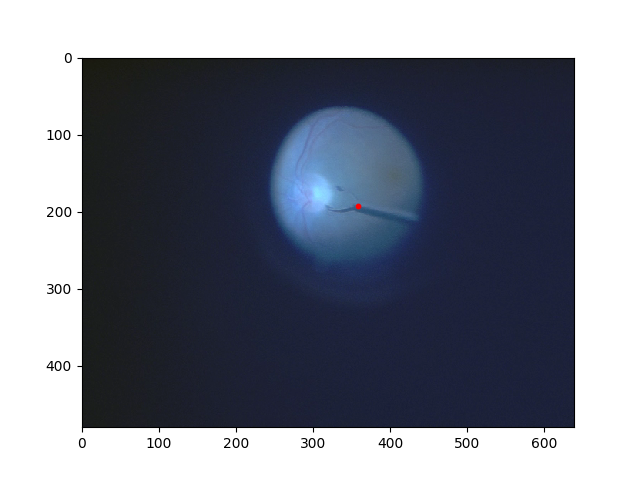
\includegraphics[width=0.25\textwidth]{figs/swa/000266.png}
    
    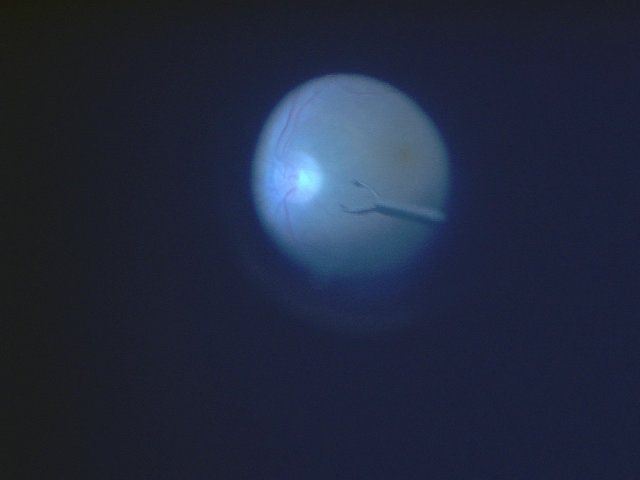
\includegraphics[width=0.25\textwidth]{figs/swa/000269.png}
    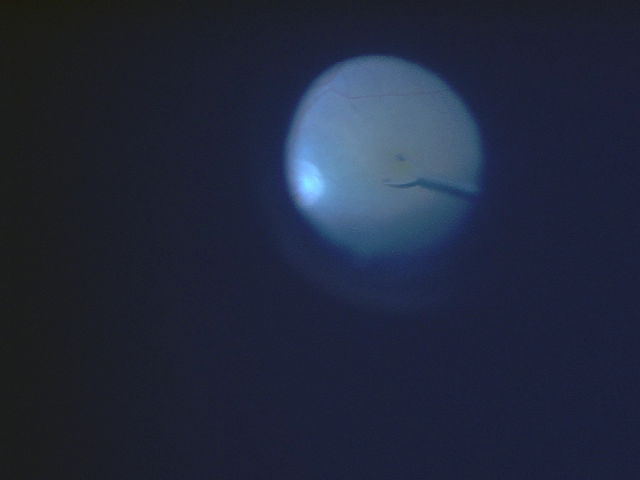
\includegraphics[width=0.25\textwidth]{figs/swa/000274.png}
    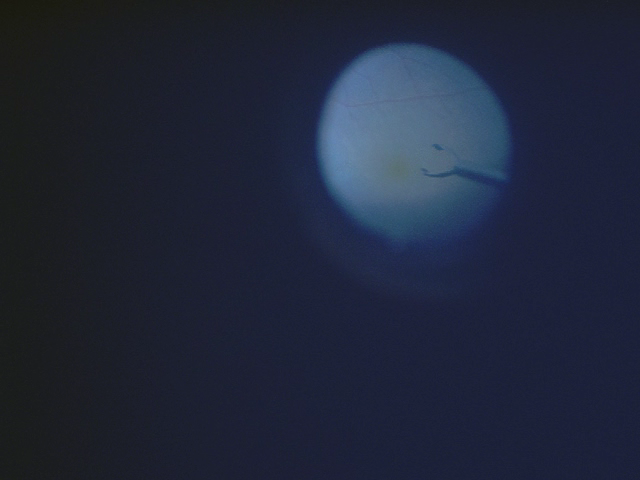
\includegraphics[width=0.25\textwidth]{figs/swa/000278.png}
    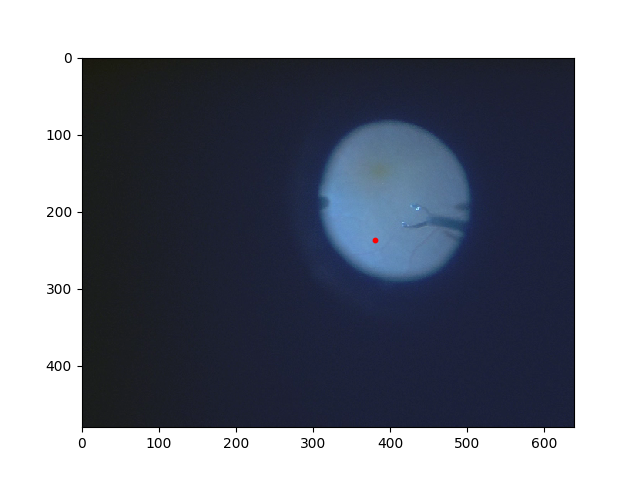
\includegraphics[width=0.25\textwidth]{figs/swa/000323.png}
\end{figure}
\end{frame}


\begin{frame}{More ideas}
\begin{itemize}
\item if correlation < 0.8 : 
\item fit color template only
\item match with previous template (not working)
\item match with any previous template (not working)
\item use negative of template (not working)
\item check with first template to find cases where match is not around the tweezer (accept cases where match is not on the right location on tweezer but correct cases where match is anywhere on the eye).
\end{itemize}
\end{frame}

\begin{frame}{Only dominant color channel A}
Filter with template cut around previous location, only dominant color channel. \\
\textbf{a}: time : 29sec / 100 images.\\
point lost tweezer, found point.
\begin{figure}
    \centering
    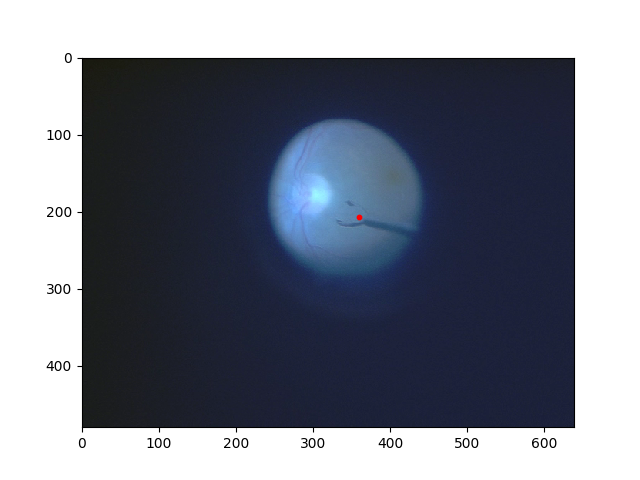
\includegraphics[width=0.25\textwidth]{figs/swa/000251.png}
    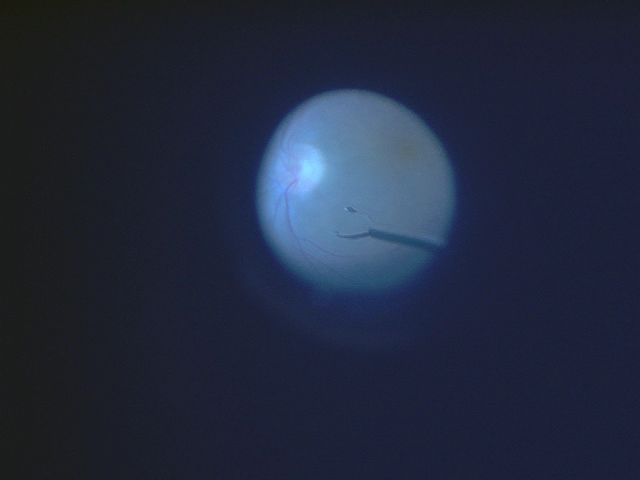
\includegraphics[width=0.25\textwidth]{figs/swa/000254.png}
    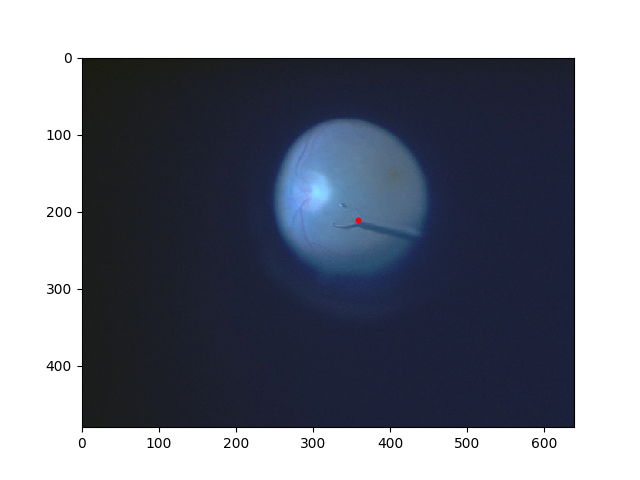
\includegraphics[width=0.25\textwidth]{figs/swa/000259.png}
    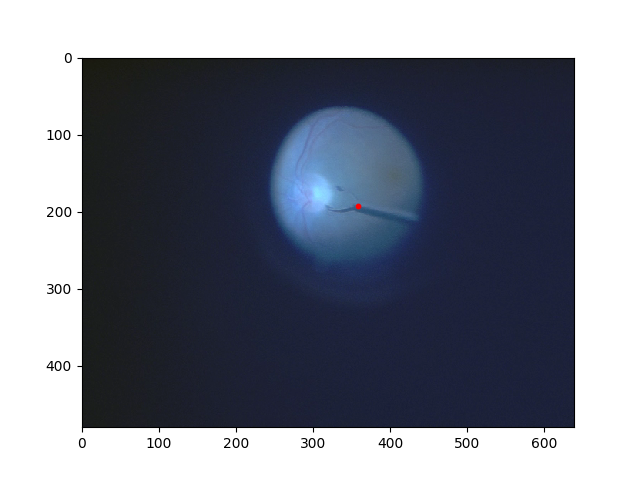
\includegraphics[width=0.25\textwidth]{figs/swa/000266.png}
    
    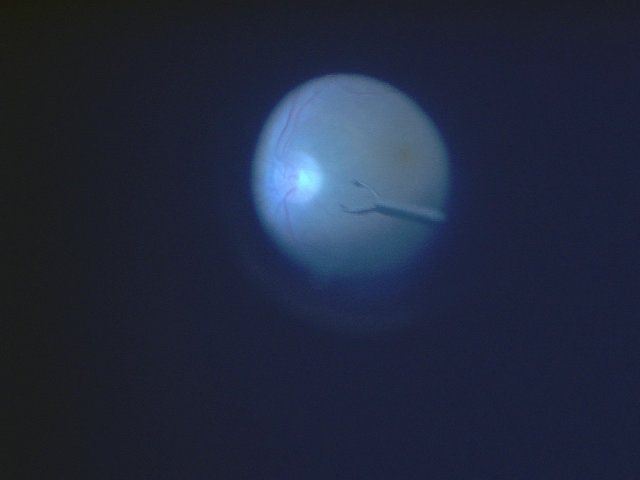
\includegraphics[width=0.25\textwidth]{figs/swa/000269.png}
    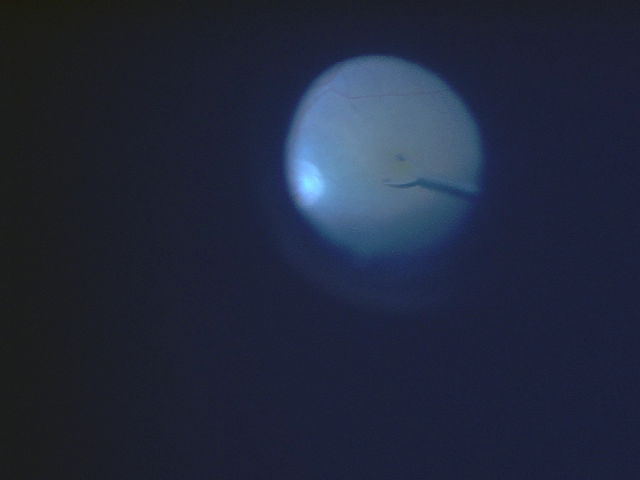
\includegraphics[width=0.25\textwidth]{figs/swa/000274.png}
    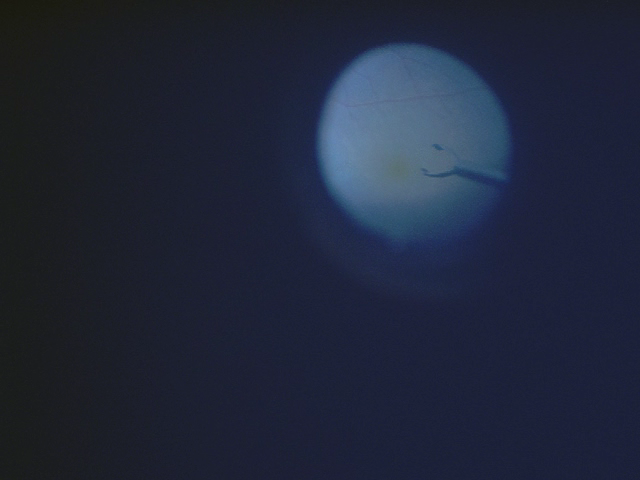
\includegraphics[width=0.25\textwidth]{figs/swa/000278.png}
    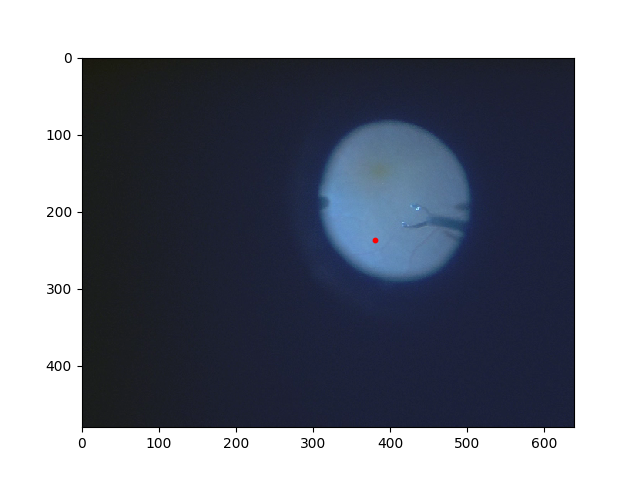
\includegraphics[width=0.25\textwidth]{figs/swa/000323.png}
\end{figure}
\end{frame}



% ---------------------------------------------------------------------------------
%\begin{frame}{Genome assembly}%{Sequence read assembly and the need for scaffolding}
%\begin{figure}
%    \centering
%    \caption*{General workflow, \tiny{Vijay Lakhujani, Biostars, 2017}}
%    \includegraphics[height=0.5\textheight]{/home/exserta/Documents/master_project_noelle/journal_club/presentation/figs/GenomeAssembly.png}
%
%    \centering
%    \includegraphics[clip, trim={50 270 210 125},height=0.25\textheight]{/home/exserta/Documents/master_project_noelle/journal_club/presentation/figs/repeats_reads.pdf}
%\end{figure}
%\end{frame}


\end{document}